\documentclass[a4paper,12pt]{article}
\usepackage[utf8]{inputenc}
\usepackage{url}
\usepackage{epsfig}
\usepackage{graphics}
\usepackage{fancyhdr}
\usepackage{subfig}
\usepackage{subfiles}

\graphicspath{{pictures/}}

\title{Sentence Generation using Two Models \\ \large{Final Project in the course DD2380 at KTH}}
\author{\hspace*{-0.5cm}
Group 61\\
\begin{tabular}{cccc}
K. Hannesson & J. Jóhannsson & E. Ahlsén & J. Andersson\\
Agust 20 & January 12 & BIRTHDATE3 & February 10 \\
hannesso@kth.se & jokull@kth.se & edvarda@kth.se & jonand8@kth.se \\
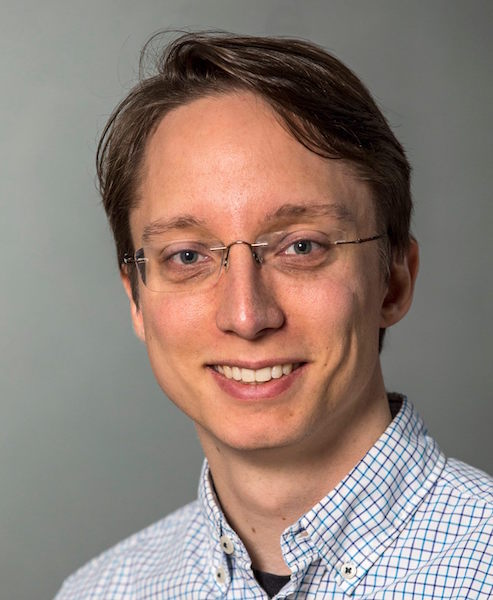
\includegraphics[width=0.13\linewidth]{photo_Kristofer} &
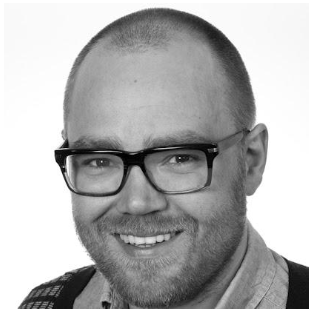
\includegraphics[width=0.13\linewidth]{photo_Jokull} &
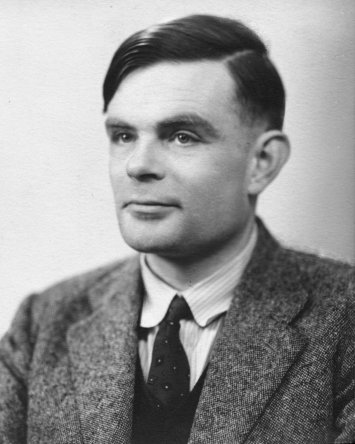
\includegraphics[width=0.13\linewidth]{Alan_Turing_photo} &
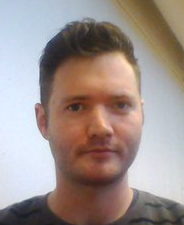
\includegraphics[width=0.13\linewidth]{photo_Jonas}
\end{tabular}}
% Normally there will not be any pictures but we want
% these so that we can connect faces to names in the course
% We also want birthdates so that we can tell people with the same
% name apart
\date{\today}

\pagestyle{fancy}
\setlength{\headheight}{15pt}
\fancyhf{}
\lhead{DD2380 ai15} % DO NOT REMOVE!!!!
\rhead{K. Hannesson, J. Jóhannsson, E. Ahlsén, J. Andersson} %% UPDATE WITH YOUR NAMES
\fancyfoot[C]{\thepage}

\begin{document}

\maketitle
\thispagestyle{fancy}

\begin{abstract}
We present two different techniques for creating n-gram models for natural language processing. Our main focus was creating sentences that would qualify as human generated sentences. We investigate how different type of smoothing affect the outcome by doing a perception test.

Our results show that using different smoothing algorithms can change the results remarkably and the way people perceive the sentences. Finally results show that XXXXXX smoothing algorithm outperform others algorithms evaluated.
\end{abstract}



\clearpage

%%%%%%%%%%%%%%%%%%%%%%%%%%%%%%%%%%%%%%%%%%%%%%%%%%%%%%%%%%%%%
%%%%%%%%%%%%%%%%%%%%%%%%%%%%%%%%%%%%%%%%%%%%%%%%%%%%%%%%%%%%%
%\section*{NOTE}
%\begin{itemize}
%
%\item The following sections are arranged in the order they would appear in a scientific paper. We think that these sections need to be there and written. However, these are only guidelines and if you think that some of these sections or subsections are irrelevant to you, please feel free to remove them. Similarly, if you want to include more sections or subsections please go ahead. Also feel free to rearrange them according to your convenience, but keeping some common sense (eg.~Introduction cannot come after Conclusions).
%
%\item \textit{Introduction, Related Works, Experimental Results, Discussions, Summary} are sections that MUST be contained.
%
%\item In the section of your \textit{Method}: please do not list your project as log book entries, please talk about the final method you want to present to us. Talk about the method scientifically or technically and not as "I did this..." "Then I tried this..." "this happened...." etc.
%
%\item Do not paste any code unless it is very relevant!
%
%\item The section \textit{Contributions} is a place to express any difference in contributions. The default assumption is that you all agree that all of you had an equal part to play in the project.
%
%\item We suggest that you try to write this as scientifically as possible and not simply like a project report. Good Luck!
%
%\item Please remove \textbf{this} NOTE section in your final report.
%
%\end{itemize}
\section{Introduction} %(1--2 pages)
\label{sec:intro}

Language models are a staple in many domains including speech recognition, optical character
recognition, handwriting recognition, machine translation, and spelling correction. The dominant technology in language modeling is n-gram models, which are straightforward to construct except for the issue of smoothing, a technique used to better estimate probabilities when there is insufficient data to estimate probabilities accurately\textbf{[Chen-Goodman]}. Many different techniques have been proposed for smoothing n-gram models. In this project we show how different smoothing techniques work and how they will affect the sentences generated.

In the following sections we will describe the difference in the models generated and how including grammar affects


**
Why was the study undertaken? What was the research question, the tested hypothesis or the purpose of the research?
**


\section{Outline}
This paper is structured as follows: In Section 1 we talk about XXXXXXX. In Section~\ref{sec:relwork} we list out how this project relates to other projects and what we did use from those projects.In Section~\ref{sec:method} we go into details about the implementation of the two models and list up which techniques we used. In Section~\ref{sec:exps} we explain how experiment were done the results.In Section~\ref{sec:summary} we summarize the most important results of this work.Finally in Section~\ref{sec:contributions} we list up the contribution of each team member to the project.

%%%%%%%%%%%%%%%%%%%%%%%%%%%%%%%%%%%%%%%%%%%%%%%%%%%%%%%%%%%%%
%%%%%%%%%%%%%%%%%%%%%%%%%%%%%%%%%%%%%%%%%%%%%%%%%%%%%%%%%%%%%
\section{Related work}
\label{sec:relwork}

\subfile{related_works}

%%%%%%%%%%%%%%%%%%%%%%%%%%%%%%%%%%%%%%%%%%%%%%%%%%%%%%%%%%%%%
%%%%%%%%%%%%%%%%%%%%%%%%%%%%%%%%%%%%%%%%%%%%%%%%%%%%%%%%%%%%%
\section{Our method}
\label{sec:method}

Should contain the following: When, where, and how was the study done? What materials were used or who was included in the study groups (patients, etc.)?

The group came up with the idea to compare two different approaches to generating text from a corpus, both including grammar but in different ways. To be able to compare them at the same level both approaches used the Brown corpus and trigrams, with fallback to bigrams allowed. A few smoothing techniques were picked for use in both approaches.
\subsection{Built in grammar model}
The first approach was to create a model that included both word and grammar information. This was achieved by generating trigrams where each word was a tuple of the word and its associated Part-Of-Speech (POS) tag. A trigram from ``the man walked'' would be (the, DET), (man, NOUN), (walked, VERB))

The distribution table contains the n-1-gram plus the tags as a key and the distribution probability of the next word. In the example above the key would be (the, DET), (man, NOUN) and that row in the table would contain the probability distribution of each word and tag that could follow that word given the corpus.

To be able to use fallback each model had 2-grams up to n-grams models. If a word/tag was not found using the n-gram model we would fallback to the n-1-gram model and so forth.

To be able to distinguish words that are in the beginning of sentence and in the end of sentence we added pseudo symbols to each sentence. The number of symbols added to the start and end of sentence would correspond n-1 in the model. Meaning that 2 start symbols were added to a trigram model.

\subsubsection{Sentence generation}
Words were picked from the model randomly given the probability of that word and the context. To find the word to start the sentence we used the start of sentence symbol. We then recursively run through the word estimation function adding a new word to the context until we get a end of sentence symbol. If a word was not found for a given context we backoff to a n-1-gram model and look for the word in that model.

\subsection{Inferred grammar model}
The second approach separated grammar and words into two models which were used in sequence to generate text. The grammar model provided what POS tag should be next, and the word model provided a word for the given tags, both using trigrams. This would take ``the man walked'' and create the trigrams (DET, NOUN, VERB) for the grammar model, and (DET, NOUN, man) and (NOUN, VERB, walked) for the grammar-word model.

\subsection{Smoothing}
The smoothing techniques chosen were:
\begin{itemize}
\item Maximum Likelihood Estimate
\item Laplace smoothing
\item Expected Likelihood Estimate
\item Simplified Good-Turing Frequency Estimation
\end{itemize}

\textbf{Maybe the sections below are not necessary?}

\subsubsection{Maximum Likelihood Estimate}
Here we will write clever stuff about this smoothing technique

\subsubsection{Laplace smoothing}
Here we will write clever stuff about this smoothing technique

\subsubsection{Expected Likelihood Estimate}
Here we will write clever stuff about this smoothing technique

\subsubsection{Simplified Good-Turing Frequency Estimation}
\subfile{smoothing-goodturing}

\subsection{Implementation}
\label{sec:impl}

We split into pairs with each pair implementing their model. We decided to go with Python 3 for the implementation because we knew the NLTK package would provide us with the necessary building blocks to construct and test the two models. These included
\begin{itemize}
\item Brown corpus
\item Treebank Part of Speech Tagger (Maximum entropy)
\item Punkt Tokenizer Models
\item Mappings to the Universal Part-Of-Speech Tagset
\item Conditional Frequency Distribution and Conditional Probability Distribution classes
\item classes for each of the above mentioned smoothing techniques
\end{itemize}

%%%%%%%%%%%%%%%%%%%%%%%%%%%%%%%%%%%%%%%%%%%%%%%%%%%%%%%%%%%%%
%%%%%%%%%%%%%%%%%%%%%%%%%%%%%%%%%%%%%%%%%%%%%%%%%%%%%%%%%%%%%
\section{Experimental results}
\label{sec:exps}

\begin{figure}[t!]%
    \centering
    \subfloat[Performance of each model as well as the real and baseline sentences]{{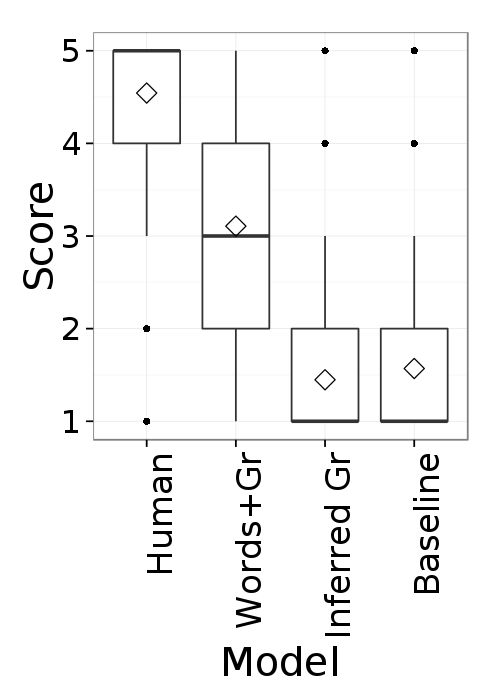
\includegraphics[width=4.5cm]{results/boxplot_resultsByModel} }}%
    \qquad
    \subfloat[Performance of each model and smoothing method]{{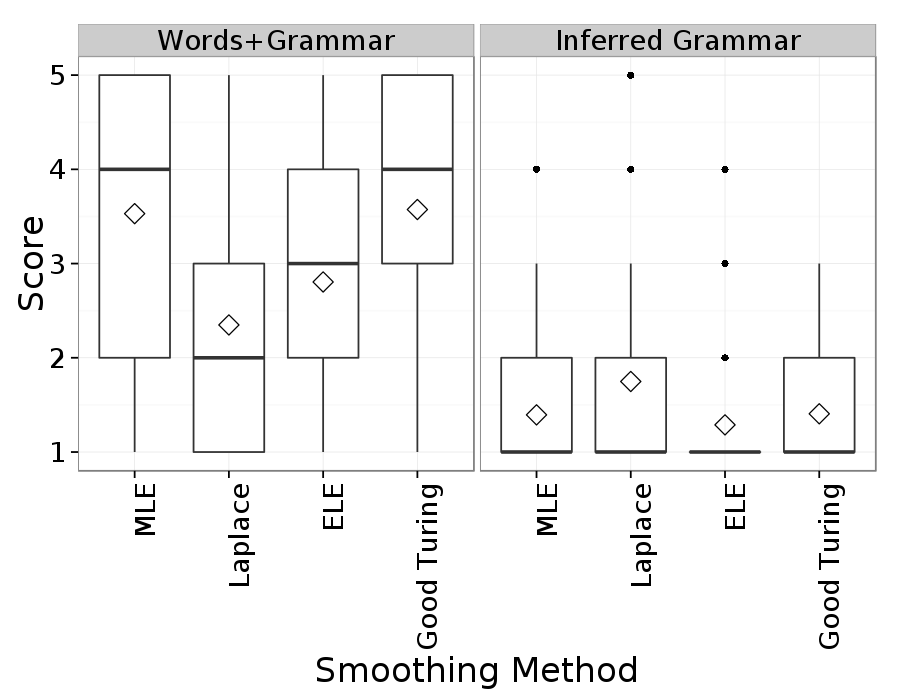
\includegraphics[width=8cm]{results/boxplot_resultsByModelAndSmoothing} }}%
    \qquad
    \caption{Model performances compared with respect to smoothing methods. Diamond represents means.}%
    \subfloat[Performance of each model as well as the real and baseline sentences]{{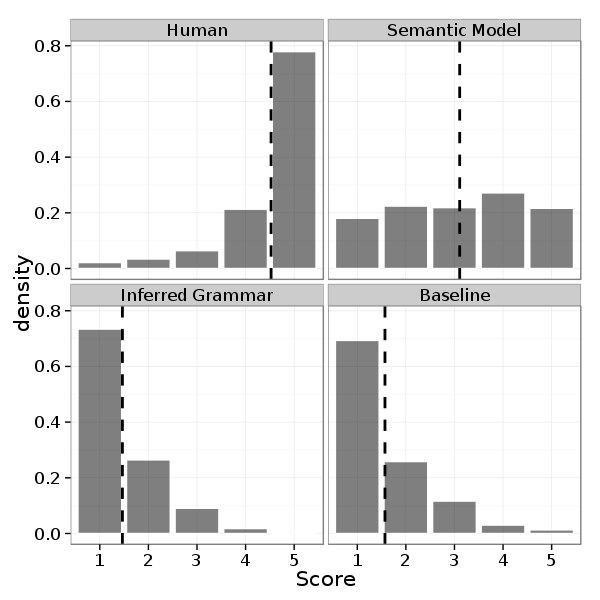
\includegraphics[width=4.5cm]{results/histogram_resultsByModel} }}%
    \qquad
    \subfloat[Performance of each model and smoothing method]{{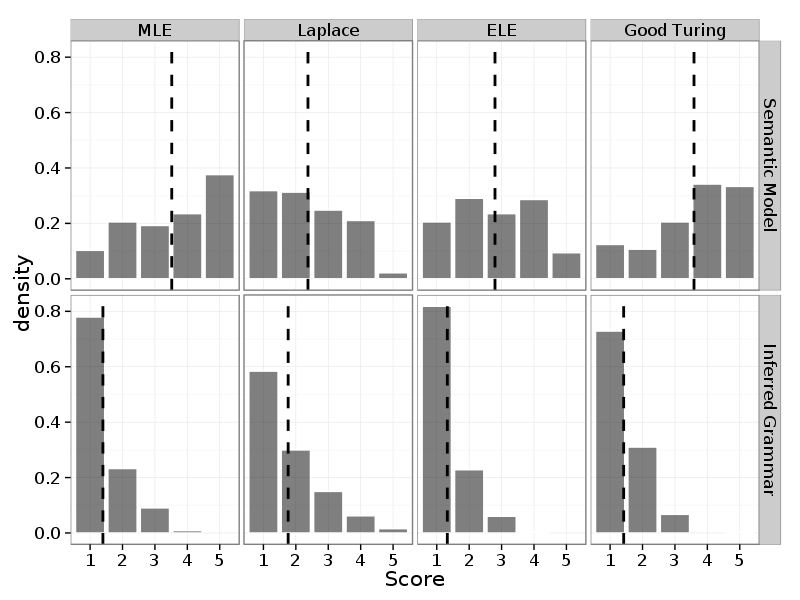
\includegraphics[width=8cm]{results/histogram_resultsByModelAndSmootingMethod} }}%
    \caption{Model performances compared with respect to smoothing methods. Dotted lines represent means.}%
    \label{fig:example}%
\end{figure}

\subsection{Experimental setup}
Each model was used to generate 5 sentences per smoothing method for a total of 40 sentences. 5 sentences were also picked from the Brown corpus. All the sentences were mixed together randomly and then added to a survey which allowed participants to rate each sentence on a scale of 1 to 5 whether it was created by a human or a computer, with 1 representing definitely a human and 5 definitely a computer. Apart from the sentence scoring we only asked if the participants were native English speakers or not. The survey solution chosen was QuestionPro.

\subsection{Experiment ...}

Here we talk about how which smoothing technique worked best for us why the results were the way they were. We also explain why the model containing the grammar was better than the inferred grammar one.

\begin{figure}
\centering
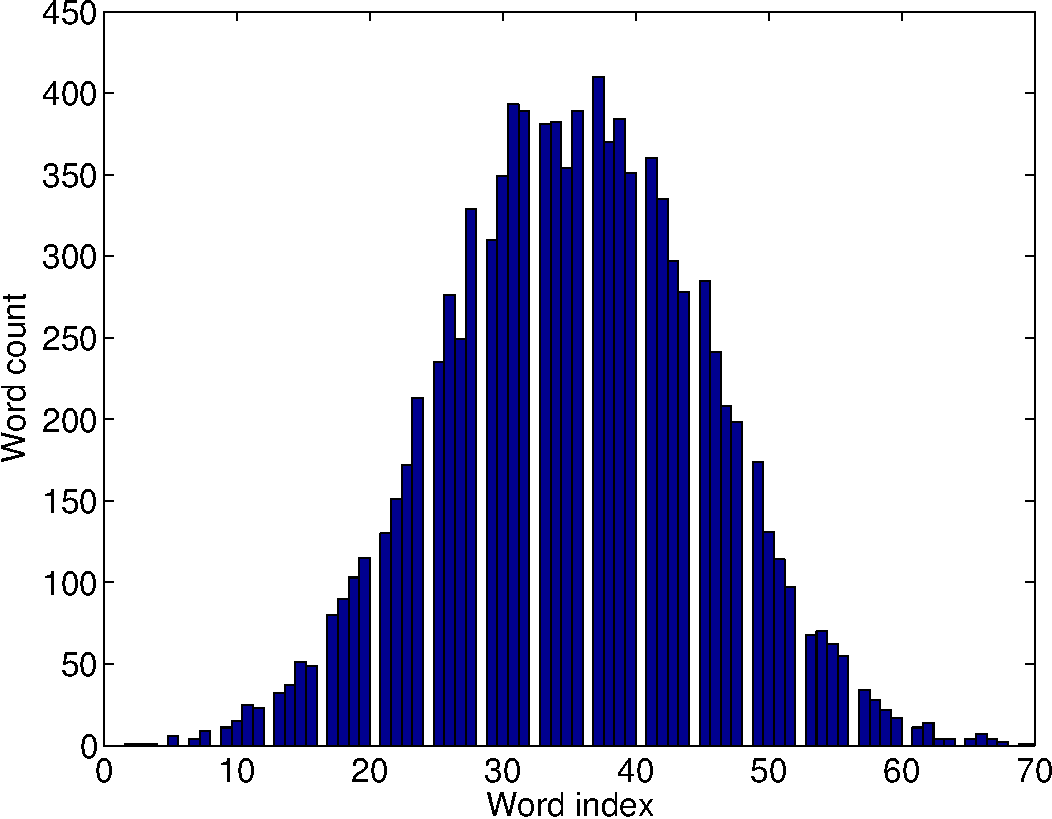
\includegraphics[width=0.8\linewidth]{histogram}
\caption{A description that makes browsing the paper easy and clearly
describes what is in the picture. Make sure that the text in the figure
is large enough to read and that the axes are labelled.}
\label{fig:histogram}
\end{figure}



\begin{table}
\begin{center}
\begin{tabular}{|c|c|c|}
\hline
Bla bla & Bla bla & Bla bla \\ \hline
42 & 42 & 42 \\ \hline
42 & 42 & 42 \\ \hline
\end{tabular}
\caption{A description that makes browsing the paper easy and clearly
describes what is in the table.}
\label{tab:results}
\end{center}
\end{table}

What answer was found to the research question; what did the study find? Was the tested hypothesis true?

%%%%%%%%%%%%%%%%%%%%%%%%%%%%%%%%%%%%%%%%%%%%%%%%%%%%%%%%%%%%%
%%%%%%%%%%%%%%%%%%%%%%%%%%%%%%%%%%%%%%%%%%%%%%%%%%%%%%%%%%%%%
\section{Summary and Conclusions}
\label{sec:summary}

In this section we present the results of our experiments. We present the performance of the algorithms tested and which of the techniques used performed best. We show the ngram count affects the sentences generated and what affect smoothing could have on a sentence generation.

We present that using

\subsection{nGram count}
We testing out different sizes 


\subsection{Smoothing}






%%%%%%%%%%%%%%%%%%%%%%%%%%%%%%%%%%%%%%%%%%%%%%%%%%%%%%%%%%%%%
%%%%%%%%%%%%%%%%%%%%%%%%%%%%%%%%%%%%%%%%%%%%%%%%%%%%%%%%%%%%%
\section{Contributions}
\label{sec:contributions}
In the beginning of the project all team members agreed that we will always work on the project together. For 5 consecutive weekends in a row the team had a NLP workshop. We started each morning with a meeting to plan  the course of our day. We than splitted up into groups of two. All team members had an equal play in the project. 

%%%%%%%%%%%%%%%%%%%%%%%%%%%%%%%%%%%%%%%%%%%%%%%%%%%%%%%%%%%%%
%%%%%%%%%%%%%%%%%%%%%%%%%%%%%%%%%%%%%%%%%%%%%%%%%%%%%%%%%%%%%
\clearpage
\bibliographystyle{plain}
\bibliography{reflist}
\end{document}
